\section{Using Amphicyon}
\label{appendix:amphicyon}
In the following section of the appendix, a short usage guide for \textsc{Amphicyon}, a tool to analyze the source code of contracts in Solidity and identify honeypots, will be provided.

To run, \textsc{Amphicyon} requires Node.js 10 and the corresponding version of yarn installed. To download all other dependencies from the npm-Repositories, use the command \texttt{yarn} launched at the base folder \texttt{amphicyon} can be used.

\subsection{Analyzing Smart Contracts}
To analyze a single smart contract, there is the command \texttt{yarn run contract:analyze <address>}. It takes a path to a file or an address as an input, and outputs its analysis result nicely formatted to the console. If an address is used, an active internet connection is required to download the contract source code from etherscan.

The output of such an execution can be seen in figure \ref{figure:appendix:amphicyon:contract:analyze}. In the first section, all inactive and not decidable classifiers are printed out, followed by the active classifiers of this analyzed contract along with a short description and a part of the source code that was relevant for this decision. In the end, the contract address is displayed together with the final score, that can range from \( 0 \) to \( \infty \), of which the later is displayed as \texttt{SURE}. The displayed value is the ratio of the probabilities for the contract being a honeypot and the contract being harmless. If this ratio is larger than \( 4 \), the contract is considered a honeypot.

Afterwards, the user is able to review the contract manually and state whether the decision made by \textsc{Amphicyon} was correct -- this information is used later to build up the classifiers of the bayesian filter.

\vspace{1em}
\begin{minipage}{\linewidth}
	\centering
	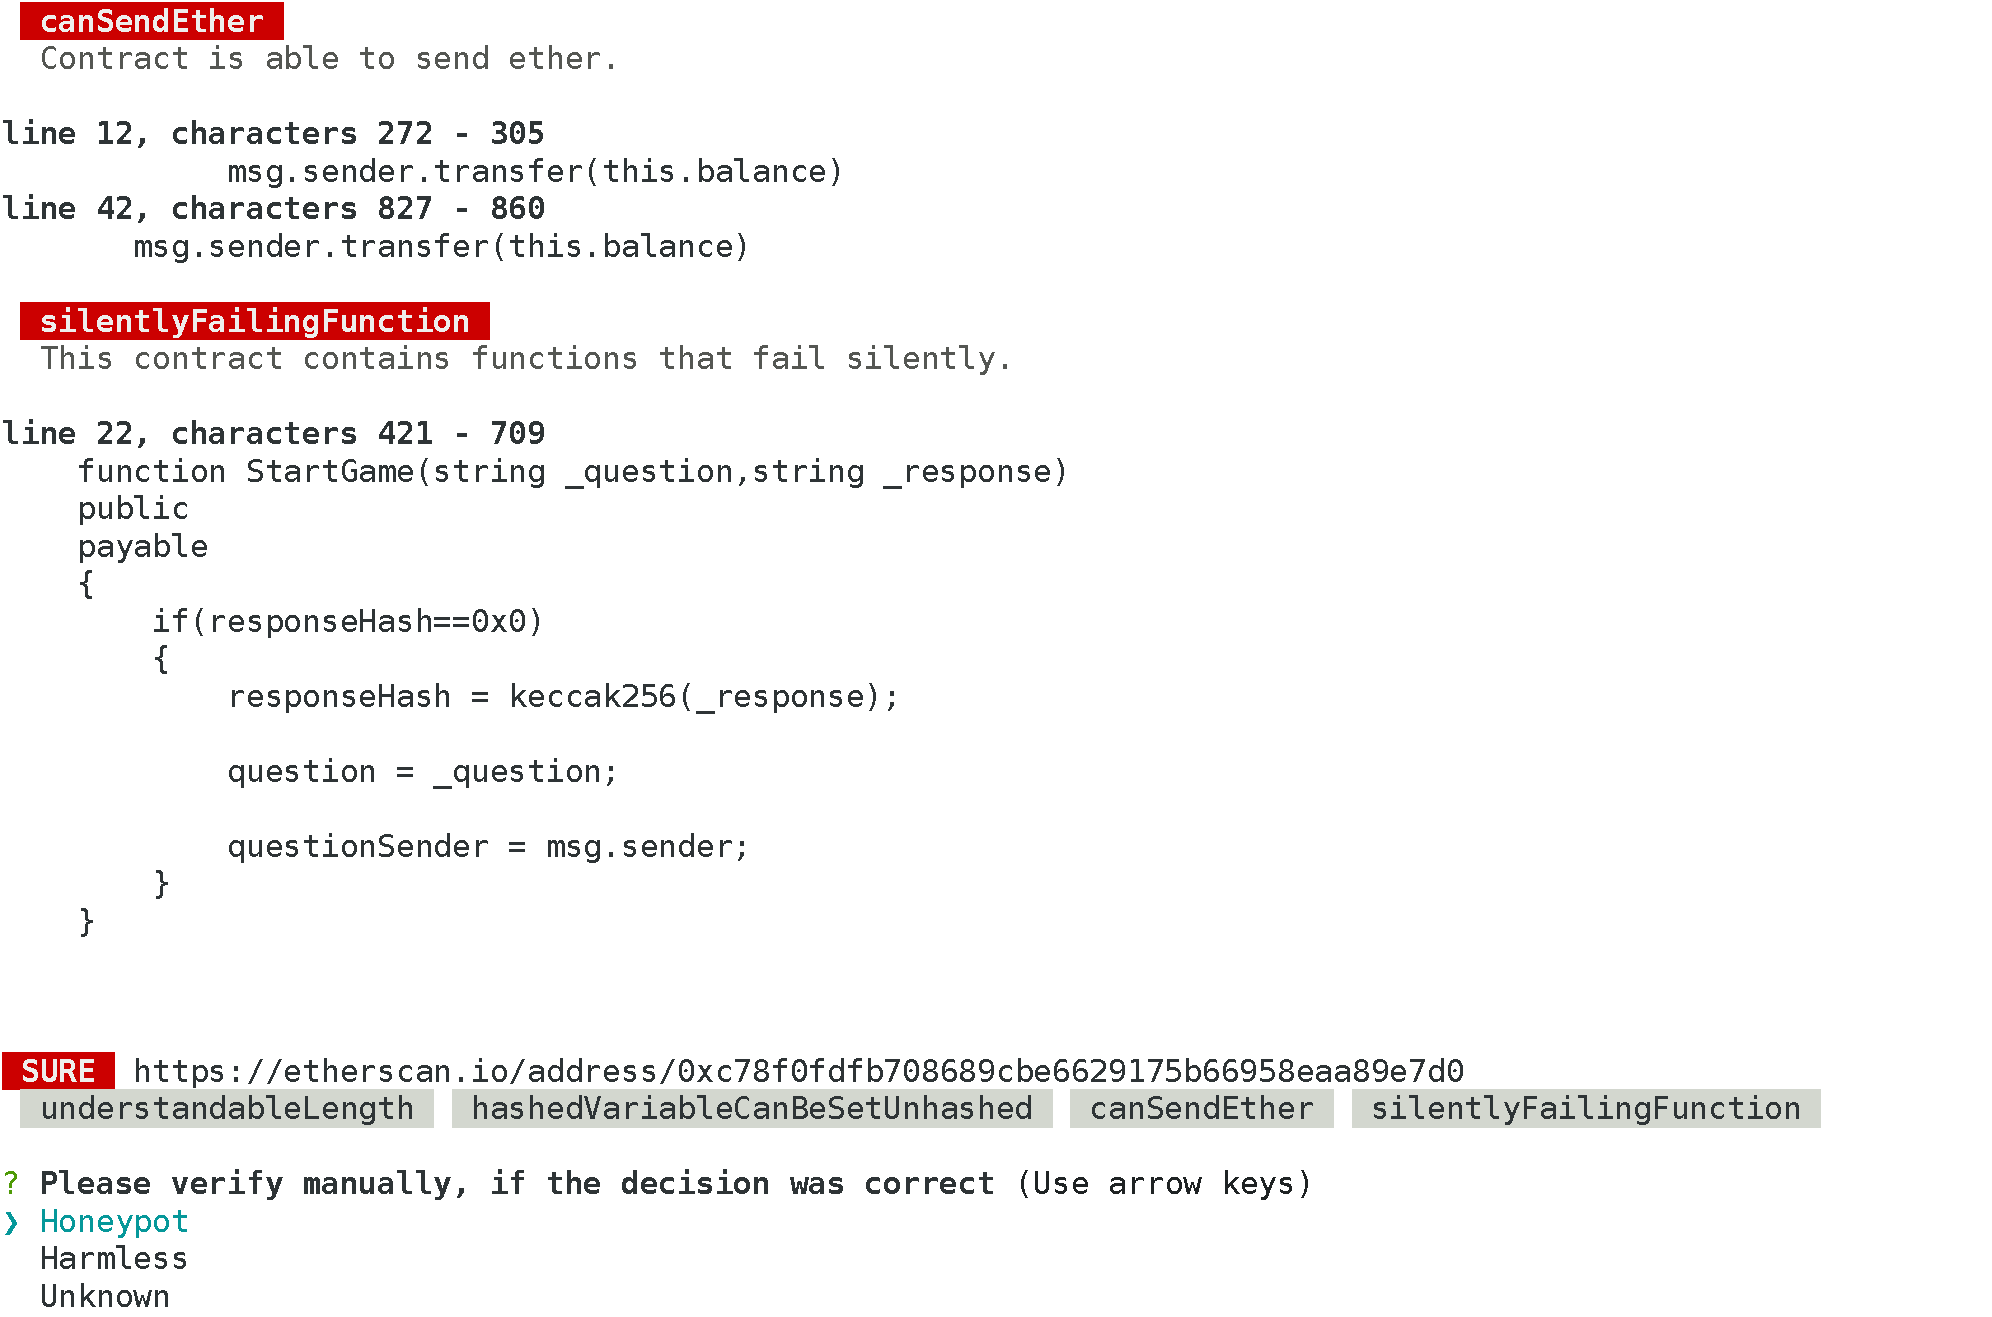
\includegraphics[width=12cm]{img/amphicyon/contract_analyze.pdf}
	\captionof{figure}[Console output for contract:analyze]{Console output for a single contract with detailed information about the found classifiers when calling \texttt{yarn run contract:analyze <address>}}
	\label{figure:appendix:amphicyon:contract:analyze}
\end{minipage}

\subsection{Bulk-Analysis}
To make the analysis of larger amounts of smart contracts possible, \textsc{Amphicyon} also has the capability to download all contracts that can be found on the "Verified Contract"-List of Etherscan. To accomplish this, the command \texttt{yarn run database:update} can be used, which will download and analyze the contracts at the latest ten pages of the list. For larger amounts, the argument \texttt{--pages=100} (here for 100 pages or 2500 smart contracts) can be used. If a contract or its analysis was already done before, the contract will not be downloaded or analyzed again.

In the data provided along with the submission, more than 8000 contracts have been downloaded. This has required more than two hours (ignoring connectivity problems), since the rate of requests per second is limited to be not blocked by Etherscan.

To display the results of the analysis of the downloaded contracts, \texttt{yarn run database:find} can be used to list all contracts the tool that were flagged as honeypots. As can be seen in the console output at figure \ref{figure:appendix:amphicyon:database:find}, along with the score all the found classifiers and the etherscan address is displayed. They are ordered by the date of the time they were downloaded.

\vspace{1em}
\begin{minipage}{\linewidth}
	\centering
	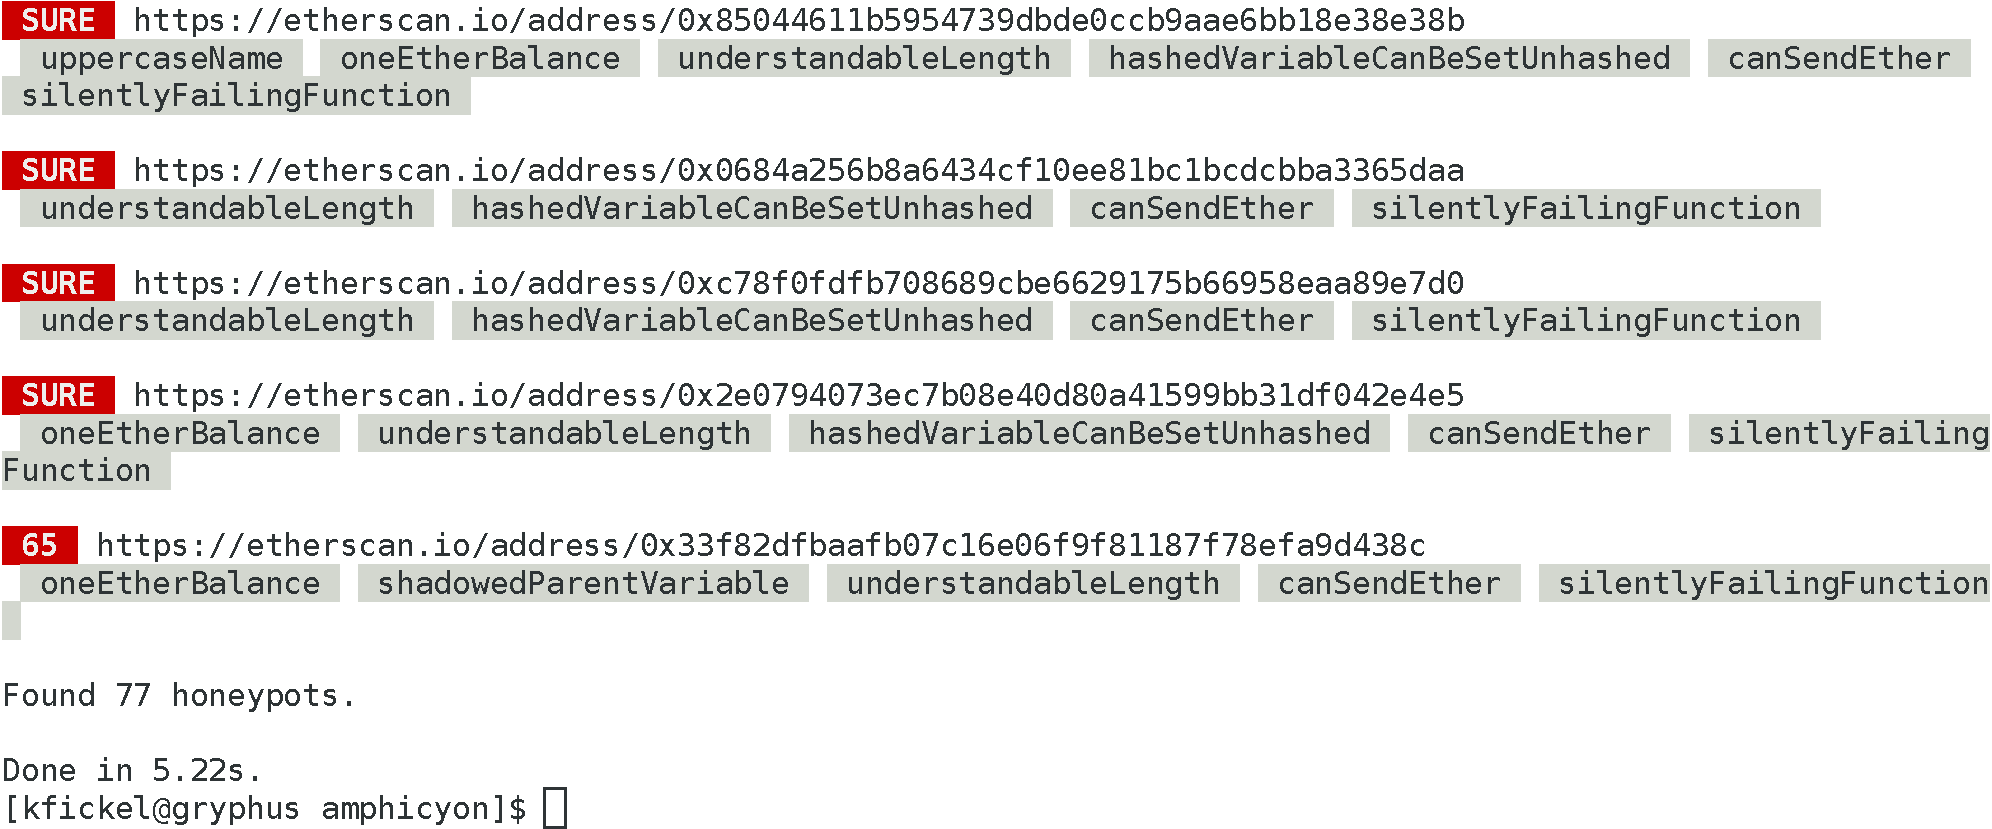
\includegraphics[width=12cm]{img/amphicyon/database_find.pdf}
	\captionof{figure}[Console output for database:find]{Console output when finding potential honeypot contracts within all downloaded contracts using \texttt{yarn run database:find}}
	\label{figure:appendix:amphicyon:database:find}
\end{minipage}

To retrieve information about the role of the classifiers, the command \texttt{yarn run database:count} can be used. It prints the amount of contracts the classifier was marked as found at, additionally separated into contracts that were later considered honeypots and those that were later considered harmless. The console output can be seen in figure \ref{figure:appendix:amphicyon:database:count}.

\vspace{1em}
\begin{minipage}{\linewidth}
	\centering
	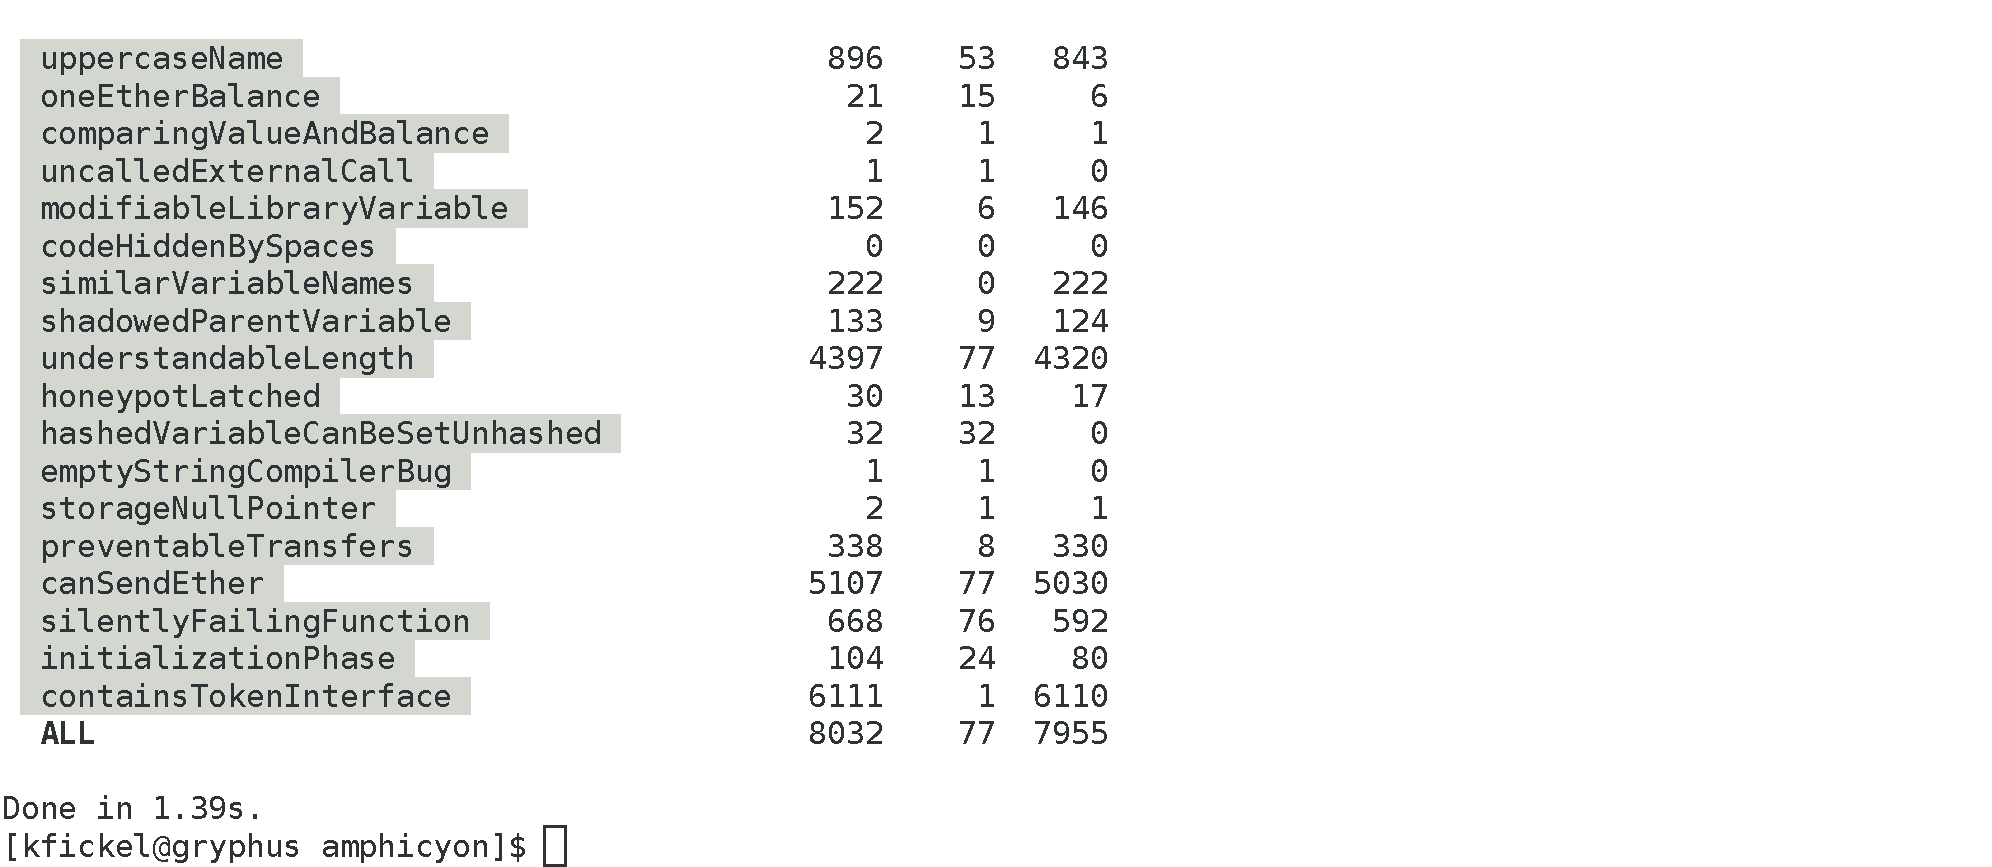
\includegraphics[width=12cm]{img/amphicyon/database_count.pdf}
	\captionof{figure}[Console output for database:count]{Console output when counting the classifier results for all downloaded contracts using \texttt{yarn run database:count}}
	\label{figure:appendix:amphicyon:database:count}
\end{minipage}

\subsection{Updating the Classifiers}
Due to the small sample size, for the final evaluation of \textsc{Amphicyon} the bayesian classifiers were build manually. The tool also implements functionality to build the classifiers based on the manual analysis results that can be added using \texttt{yarn run contract:analyze}: By calling \texttt{yarn run classifiers:update}, the contracts with manual decisions will be downloaded, analyzed and counted to build a valid classifier file that can be used to replace the default file.

\pagebreak{}
